\documentclass[prd,aps,twocolumn,superscriptaddress,tightenlines,nofootinbib,floatfix,preprintnumbers,10pt]{revtex4-1}
\usepackage{amsmath,amssymb}
\usepackage{bm}
\usepackage{comment}
\usepackage{graphicx}
\usepackage{color}
\usepackage{cancel}
\usepackage{tikz}
\usetikzlibrary{shapes.misc}
\usepackage{CJKutf8}

\usepackage{hyperref}
\hypersetup{
    colorlinks=true,       % false: boxed links; true: colored links
    linkcolor=blue,          % color of internal links
    citecolor=blue,        % color of links to bibliography
    filecolor=blue,      % color of file links
    urlcolor=blue           % color of external links
}
\allowdisplaybreaks


% Greek Letters
\def\a{{\alpha}}
\def\b{{\beta}}
\def\d{{\delta}}
\def\D{{\Delta}}
\def\e{{\epsilon}}
\def\g{{\gamma}}
\def\G{{\Gamma}}
\def\k{{\kappa}}
\def\l{{\lambda}}
\def\L{{\Lambda}}
\def\m{{\mu}}
\def\n{{\nu}}
\def\w{{\omega}}
\def\O{{\Omega}}
\def\S{{\Sigma}}
\def\s{{\sigma}}
\def\t{{\tau}}
\def\th{{\theta}}
\def\x{{\xi}}

\def\ol#1{{\overline{#1}}}

%slash's
\def\Dslash{D\hskip-0.65em /}
\def\dslash{{\partial\hskip-0.5em /}}
\def\vslash{{\rlap \slash v}}
\def\qbar{{\overline q}}

% Jargon
\def\CPT{{$\chi$PT}}
\def\QCPT{{Q$\chi$PT}}
\def\PQCPT{{PQ$\chi$PT}}
\def\tr{\text{tr}}
\def\str{\text{str}}
\def\diag{\text{diag}}
\def\order{{\mathcal O}}
\def\vit{{\it v}}
\def\vD{\vit\cdot D}
\def\am{\alpha_M}
\def\bm{\beta_M}
\def\gm{\gamma_M}
\def\smb{\sigma_M}
\def\smt{\overline{\sigma}_M}
\def\tb{{\tilde b}}

\def\mc#1{{\mathcal #1}}

% Fields
\def\Bbar{\overline{B}}
\def\Tbar{\overline{T}}
\def\cBbar{\overline{\cal B}}
\def\cTbar{\overline{\cal T}}
\def\pq{(PQ)}


\def\eqref#1{{(\ref{#1})}}

\newcommand{\glasgow}{
	School of Physics and Astronomy, 
    University of Glasgow, 
    Glasgow G12 8QQ, UK
	}
\newcommand{\jlab}{
	Theory Center, 
	Thomas Jefferson National Accelerator Facility, 
	Newport News, VA 23606, USA
	}
\newcommand{\jlabcomp}{
	Scientific Computing Group, 
	Thomas Jefferson National Accelerator Facility, 
	Newport News, VA 23606, USA
	}
\newcommand{\lblnsd}{
	Nuclear Science Division,
    Lawrence Berkeley National Laboratory,
	Berkeley, CA 94720, USA
	}
\newcommand{\wm}{
	Department of Physics,
	The College of William \& Mary,
	Williamsburg, VA 23187, USA
	}
\newcommand{\ucb}{
	Department of Physics,
	University of California,
	Berkeley, CA 94720, USA
}
\newcommand{\ithems}{
	Interdisciplinary Theoretical and Mathematical Sciences Program (iTHEMS), RIKEN,
	2-1 Hirosawa, Wako, Saitama 351-0198, Japan
}
\newcount\hour \newcount\hourminute \newcount\minute
\hour=\time \divide \hour by 60
\hourminute=\hour \multiply \hourminute by 60
\minute=\time \advance \minute by -\hourminute
\newcommand{\mydate}{\ \today \ - \number\hour :\number\minute}

\begin{document}


\title{The Slope of Form Factors from Lattice QCD}

\author{Chia~Cheng~Chang \begin{CJK*}{UTF8}{bsmi}(張家丞)\end{CJK*}}
\affiliation{\lblnsd}

\author{David~Richards}
\affiliation{\jlab}

\author{Chris~Bouchard}
\affiliation{\glasgow}

\author{Kostas~Orginos}
\affiliation{\wm}
\affiliation{\jlab}




%\date{\mydate}

\begin{abstract}
% This is Lattice2016 abstract
Momentum-space derivatives of matrix elements can be related to their
coordinate-space moments through the Fourier transform. We derive
these expressions as a function of momentum transfer $Q^2$ for
asymptotic in/out states consisting of a single hadron. We calculate
corrections to the finite volume moments by studying the spatial
dependence of the lattice correlation functions. This method permits
the computation of not only the values of matrix elements at momenta
accessible on the lattice, but also the momentum-space derivatives,
providing a priori information about the $Q^2$ dependence of form
factors. As a specific application we use the method, at a single
lattice spacing and with unphysically heavy quarks, to directly obtain
the slope of the isovector form factor at various $Q^2$, whence the
isovector charge radius. The method has potential application in the
calculation of any hadronic matrix element with momentum transfer,
including those relevant to hadronic weak decays.
\end{abstract}
\maketitle

%%%%%%%%%%%%%%%%%%%%%%%%%%%%%%%%%


\section{Introduction\label{sec:intro}}
Answers to some of the deepest mysteries of nature may be uncovered
through fundamentally understanding how protons and neutrons, the
basic building blocks of our world, interact with the universe. The
lattice QCD community has contributed to our understanding of the
strength of these interactions by direct calculations of form
factors. In this work, we propose a method to directly calculate the
slope of these form factors, which shed light on new ways to test our
current understanding of the Standard Model.

\subsection{On the radius of the proton}
The charged leptons are fundamental (point-like) particles in the
Standard Model of particle physics, with identical coupling strengths
to the electroweak currents, and only differ in mass between the three
generations. This Standard Model paradigm, known as \textit{lepton
  universality}, is however, in tension with recent experimental
observations of the proton charge radius~\cite{Carlson:2015jba}. In
particular, measurement from muonic Hydrogen~\cite{nature09250}
resulted in a 4\% smaller proton radius when compared to the CODATA
average from 24 transition frequency measurements of atomic
Hydrogen~\cite{RevModPhys.80.633}, in tension at 4 standard
deviations. This discrepancy hints at the possibility that the
electron and muon may differ fundamentally in ways unaccounted for by
the Standard Model. Recently, evidence of possible resolution to the
proton radius puzzle was provided by an updated measurement of the
2S-4P transition frequency~\cite{Beyer79} that is consistent with the
muonic Hydrogen measurement. However, a recent update on the 1S-3S
transition frequency~\cite{fleurbaey:tel-01633631} continues to
re-enforce the discrepancy between atomic and muonic
experiments.

Electron scattering results continue to exhibit the long standing
discrepancy with muonic Hydrogen~\cite{Sick:2018fzn}. Due to the vast
number of transition frequencies from Lamb shift measurements, and
tension from the electron scattering result, resolution to the charge
radius puzzle may still require considerable additional effort from
experimentalists. Furthermore, the ratio of semi-leptonic
$B\rightarrow D^{(*)}\ell\bar{\nu}$ decays to the electron and tau
final states is also observed to be in tension with the Standard Model
prediction at 4 standard deviations~\cite{Ciezarek:2017yzh}, lending
evidence that the discrepancy seen in the proton radius may in fact be
a result of new physics.

While the measurement of the proton radius is very challenging, its
definition is straightforward from a theory stand point. Specifically,
the charge radius of the proton $\langle r \rangle$ is defined through the $Q^2$
derivative of the Sach's form factor $G_E(Q^2)$
evaluated at zero-momentum transfer
\begin{equation}
  \left. \frac{\partial G_E(Q^2)}{\partial Q^2} \right| = -\frac{1}{6}
    \langle r^2 \rangle = \left. \frac{\partial F_1(Q^2)}{\partial
      Q^2}\right| - \frac{F_2(0)}{4 M^2},\label{eq:radius}
\end{equation}
where $F_1(Q^2)$ and $F_2(Q^2)$ are the Dirac and Pauli form factors,
and $M$ is the proton mass.
These form factors are then defined in terms of the matrix elements of
the electromagnetic current
\begin{eqnarray}
\lefteqn{\langle N(\vec{p}_f \mid V_{\mu}(0) \mid N(\vec{p}_i \rangle
  =} \nonumber \\
& &  \bar{u}(\vec{p}_f) \left[ F_q(q^2) \gamma_\mu + \sigma_{\mu\mu}
    q_\nu \frac{F_2(q^2)}{2 M} \right] u(\vec{p}_i)
\end{eqnarray}
where $\vec{q} = \vec{p}_f - \vec{p}_i$ is the three-momentum transfer
and $Q^2 = (E_f - E_i)^2 - \vec{q}^2$ is the four-momentum transfer
entering into eqn.~\ref{eq:radius}.  The calculation of both the
isovector and isoscalar electromagnetic form factors through the
determination of the matrix element defined above is a
well-established program in lattice QCD, with extensive studies aimed
at controlling the systematic uncertainties that enter into their
evaluation.

Current lattice QCD determinations of the radius, however, remain
problematical, because the derivative is extracted from modeling the
$Q^2$ dependence of $F_1(Q^2)$ from calculations at the discrete
values of momentum accessible in a finite volume.  Indeed, the
problems encountered in extracting the charge radius from lattice
calculations of the form factor in some respects mirror those in
electron-scattering experiments, where the form factor is computed for
a descrete, albeit closely spaced, set of finite $Q^2$, and the need
to include dispersive methods in the analysis of the form factors over
the values of $Q^2$ probed in experiment has been
emphasised\cite{Alarcon:2018irp}.  Thus lattice calculations are
susceptible to two major problems: the model dependence that
introduces uncontrolled systematic errors, and that the smallest
non-zero momentum is too large to perform a controlled extrapolation
of the slope at zero-momentum since accessing small momentum in finite
volumes requires very large lattices that are prohibitively expensive.

\subsection{On the origin of matter}
One of the outstanding mysteries of our universe lies in quest to
understand the origin of matter, or more specifically the origin of
the matter-antimatter asymmetry that we observe today. There is
tantalizing evidence for possible sources of \textit{leptogenesis}
recently revealed at the \textit{Tokai-2-Kamioka} (T2K) long-baseline
neutrino experiment~\cite{Abe:2017uxa}, where CP conservation in the
neutrino sector is excluded at 90\% confidence.  Future long-baseline
neutrino experiments including the \textit{Deep Underground Neutrino
  Experiment} (DUNE), and the detector upgrade to Hyper-Kamiokande
(T2HK) aims to provide more precise neutrino oscillation measurements
in order to further resolve the neutrino CP-violating
phase. Additionally, cost-effective projects such as \textit{CHerenkov
  detectors In mine PitS} (CHIPS)~\cite{Adamson:2013xka}, a water
Cherenkov detector designed to be approximately 5 times larger than
Super-Kamiokande, is planned with the intention to ultimately run off
the DUNE beamline, providing a cost-efficient way to improve knowledge
on neutrino parameters including the CP violating phase.

In order to fully benefit from the advances of next generation
neutrino experiments, the theoretical description of neutrino
scattering must also be made more precise through improving the
current determination of the nucleon axial form factor $F_A(Q^2)$. The
axial form factor parameterizes the strength in which the weak current
couples to the nucleon, and consequently governs the neutrino
scattering cross-section off nuclear targets in the regime of
quasi-elastic scattering. There is currently a 1--2\% uncertainty on
the determination of the cross-section~\cite{Adams:2013qkq} that is
dominated by the hadronic uncertainty on the axial form factor at
small momentum transfer up to approximately
1~GeV~\cite{Day:2012gb}. Similar to the determination of the charge
radius, the shape of the form factor is often derived from the model
dependent dipole ansatz. Recent progress in lattice QCD has
demonstrated control at the percent-level over the axial form factor
at zero-momentum transfer~\cite{Chang:2017oll}. The method introduced
in this paper is extensible to calculations of the slope at non-zero
momentum transfer and paves a way for controlling the full momentum
dependence of the form factor at the same level of precision.

\subsection{Overview}

The remainder of the paper is laid out as follows.  In the next
section, we introduce moment methods in which time-sliced
correlation functions are weighted by moments of a spatial coordinate,
and demonstrate how these methods enable the momentum-dependent slope of form factors to
be directly computed at the momenta allowed on the lattice.  We
describe previous applications of the method, and then describe how
these methods can be used to determine the slope of the nucleon
electromagnetic form factors at $Q^2 = 0$, and hence the charge radius
of the nucleon.  We concluded the section by describing our analysis
method, emphasising in particular the need to allow for excited-state
contributions to the correlation functions, and the anticipated
finite-volume behaviour.

In Section~\ref{sec:results}, we present the application of the method
to the isovector charge radius of the nucleon.  We begin by describing
the parameters of the ensembles used in our calculation, emphasising
the need to understand the dependence of the results on the spatial
volume of our lattices.  We present results for the charge radius for
several separations between the nucleon source and nucleon sink,
demonstrating the need to include the contribution of excited nucleon
states in our fitting procedure.  The calculation is performed at
unphysically large values of the pion mass, and at a relatively coarse
lattice spacing.  We conclude with an program of future work, and of
other applications, including to the determination of the axial-vector
charge radius.

We emphasise that the aim of this paper is not to provide a direct
calculation of the charge radius that can confront experiment, but
rather to present a method that can address one of the main systematic
uncertainties that plague present calculations.

\section{Moments of correlation functions}
{\color{red} This part is only slightly reworded from the
  proceedings. I am pointing this out in case any one thinks it's a
  problem.}  Position-space moment methods was first introduced to
calculate the slope of the Isgur-Wise function $\xi (w)$ at
zero-recoil, in order to interpret experimental results near
zero-recoil for $B \rightarrow D$ semi-leptonic
decays~\cite{Lellouch:1994zu}, and later adapted to calculate the
slope of the energy-momentum tensor form factor, yielding the angular
momentum contribution to the spin of the
nucleon~\cite{Mathur:1999uf,Gadiyak:2001fe}. Recently, there is
revitalized interest in applying moment methods to calculate the
hadronic vacuum polarization~\cite{Chakraborty:2016mwy,Blum:2016xpd},
and efforts to directly determine the anomalous magnetic moment of the
nucleon and radii in nuclear physics~\cite{Alexandrou:2016rbj}. In
parallel, momentum-space derivative methods are also being explored to
access similar nucleon structure calculations such as the anomalous
magnetic moment and various nucleon
radii~\cite{deDivitiis:2012vs,Tiburzi:2014yra}. In this work, we
present a coordinate-space method that directly calculates the slope
of single particle form factors with respect to the squared
momentum-transfer at any lattice accessible momenta.

\subsection{Formalism}
\begin{figure}[t]
	\centering
	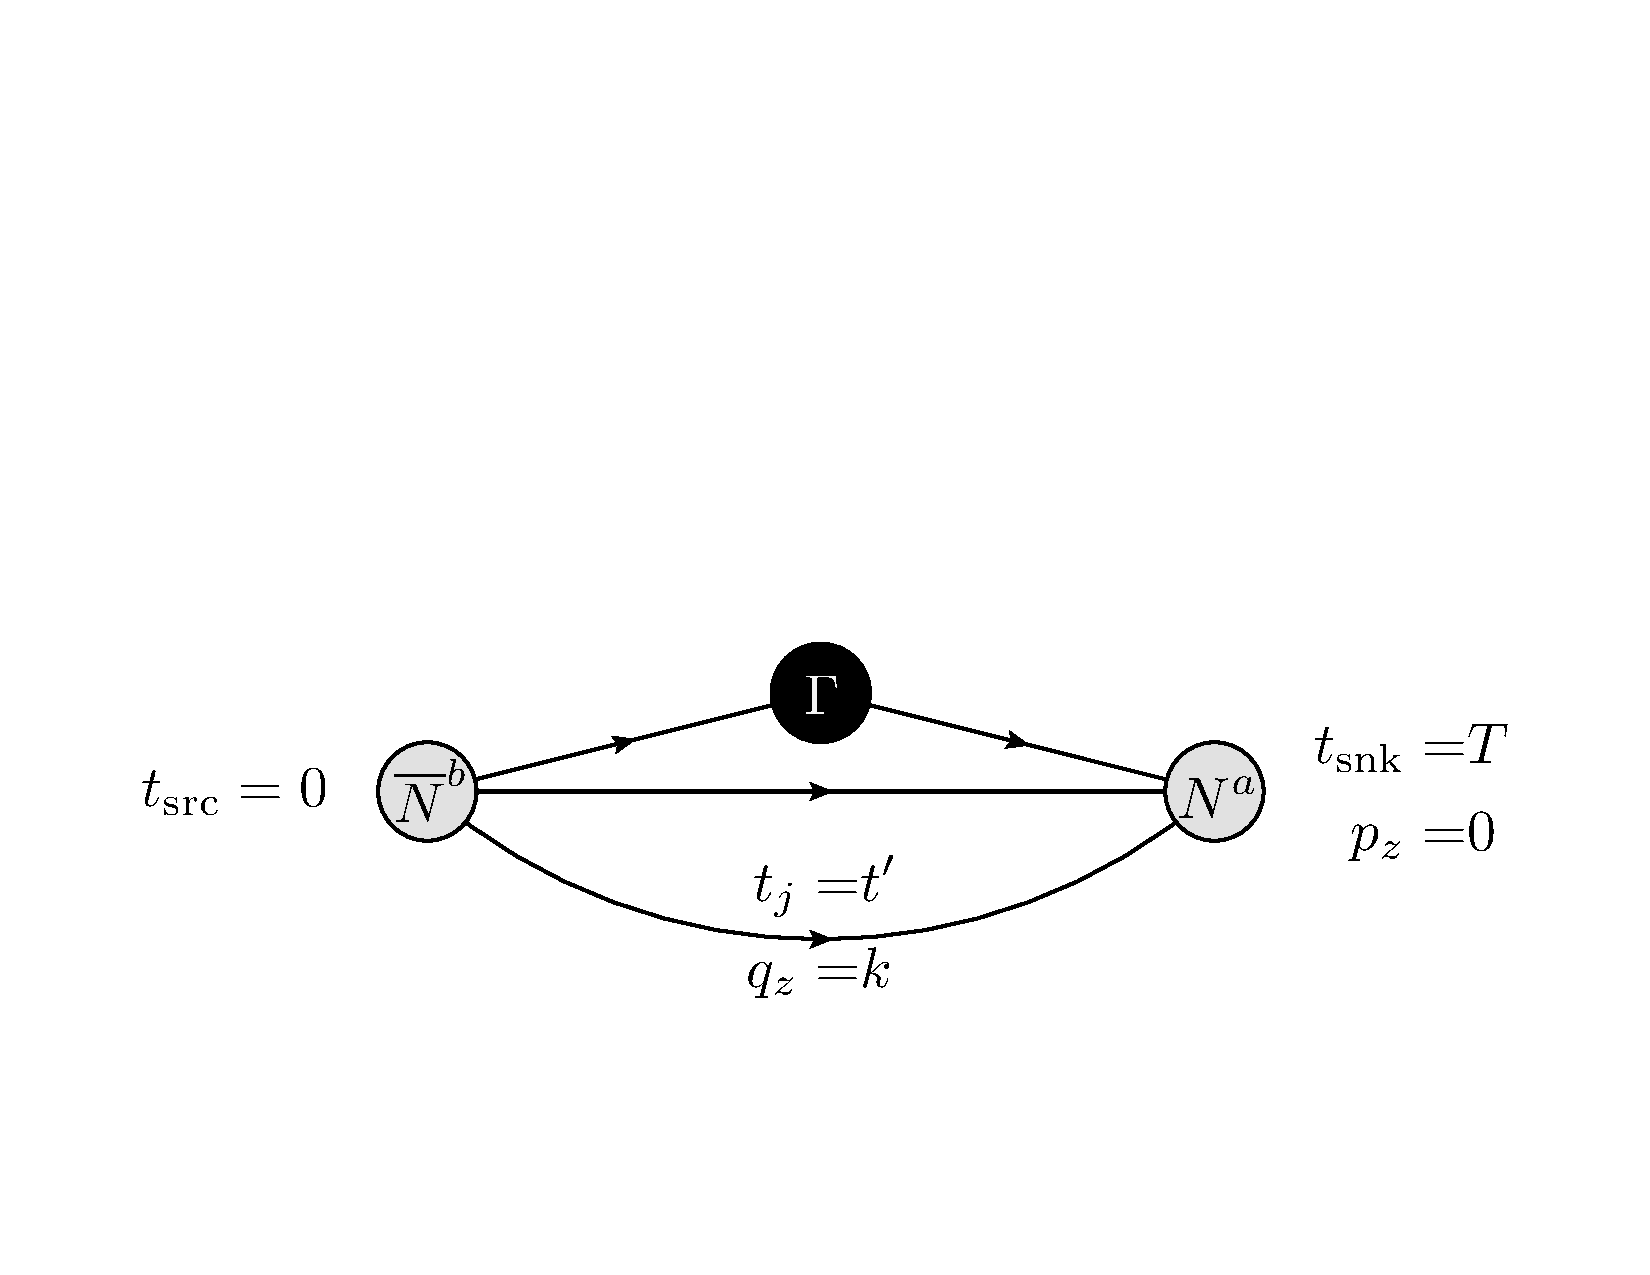
\includegraphics[width=\columnwidth]{./cropped_kinematics.pdf}
	\caption{Kinematics of the three-point correlator with baryon initial and final states. We work in the rest frame of the final hadron. The diagram for semi-leptonic decays of mesons involves only one spectator quark, but involves the same kinematics. {\color{red} Change $a$ and $b$ to say src and snk.}}
	\label{fig:3pt_kinematics}
\end{figure}
{\color{red} Some more self-plagiarism.}
\subsubsection{Three-point correlation function}
Given a three-point correlation function with the initial state at rest, and current insertion with three-momentum $k$, where $k$ points in the $z$-direction without loss of generality, as shown in Fig.~\ref{fig:3pt_kinematics}, the three-momentum-projected three-point has the general form,
\begin{align}
C^{\text{3pt}}(t, t^\prime) = \sum_{\vec{x},\vec{x}^\prime} \left<N^{\mathrm{snk}}_{t,\vec{x}}\Gamma_{t^\prime,\vec{x}^\prime} \overline{N}^{\mathrm{src}}_{0,\vec{0}}\right> e^{-ikx^\prime_z},
\label{eq:3pt}
\end{align}
translational invariance allows us to shift the source to the origin
$\vec{x}_{\mathrm{src}} = 0$ and the sink to $\vec{x}\equiv
\vec{x}_{\mathrm{snk}} - \vec{x}_{\mathrm{src}}$. Since the sink has
zero three-momentum, the only momentum dependence left is at the
current insertion. The operators $N^{\mathrm{src}}$ and
$N^{\mathrm{snk}}$ are the source and sink interpolation operators
respectively, allowing for different choices of the nucleon
interpolating operator~\cite{Basak:2005ir,Basak:2007kj} and operator
smearing profiles. The operator $\Gamma$ is a generic current
insertion at position $\vec{x}^\prime\equiv
\vec{x}_J-\vec{x}_{\text{src}}$.

The derivative of the three-point correlator with respect to $k^2$ follows,
\begin{align}
C^\prime_{\text{3pt}}(t, t^\prime)
=& \sum_{\vec{x},\vec{x}^\prime} \frac{-x^\prime_z}{2k}\sin\left(kx^\prime_z\right) \left<N^{\mathrm{snk}}_{t,\vec{x}}\Gamma_{t^\prime,\vec{x}^\prime} \overline{N}^{\mathrm{src}}_{0,\vec{0}}\right>, 
\label{eq:3ptmoment}
\end{align}
where in Eq.~(\ref{eq:3ptmoment}), the cosine component vanishes due to symmetry. In the limit of zero momentum, the $k^2 \rightarrow 0$ limit of the integrand is given by L'H\^opital's rule,
\begin{align}
\lim_{k^2 \rightarrow 0} C^\prime_{\text{3pt}}(t, t^\prime) = & \sum_{\vec{x},\vec{x}^\prime}\frac{-x^{\prime 2}_z}{2}\left<N^{\mathrm{snk}}_{t,\vec{x}}\Gamma_{t^\prime,\vec{x}^\prime} \overline{N}^{\mathrm{src}}_{0,\vec{0}}\right>.
\label{eq:3ptmoment0}
\end{align}

While it is tempting to think of Eq.~(\ref{eq:3ptmoment0}) as having an $x^{\prime 2}_z$ moment, it is clear from Eq.~(\ref{eq:3ptmoment}), that a single derivative contributes only a single factor of $x^{\prime}_z$. The second factor of $x^{\prime}_z$ only appears in the $k^2\rightarrow 0$ limit and should not be thought as a position-space moment resulting from a momentum-space derivative.

\subsubsection{Two-point correlation function}
Analogously, given a two-point correlator with three-momentum $k$ in the $z$-direction,
\begin{align}
C_{\text{2pt}}(t) = \sum_{\vec{x}} \left< N^{\mathrm{snk}}_{t,\vec{x}}\overline{N}^{\mathrm{src}}_{0,\vec{0}}\right> e^{-ikx_z},
\label{eq:2pt}
\end{align}
the derivative of the two-point correlator with respect to $k^2$ follows,
\begin{align}
C^\prime_{\text{2pt}}(t)
% \equiv & \frac{\partial}{\partial k^2} C_{\text{2pt}}(t),  \nonumber\\
= & \sum_{\vec{x}}\frac{-x_z}{2k} \sin\left(kx_z\right) \left<N^{\mathrm{snk}}_{t, \vec{x}}\overline{N}^{\mathrm{src}}_{0,\vec{0}} \right>.
\label{eq:2ptmoment}
\end{align}
 Analogous to the moment of the three-point correlator, the cosine contribution vanishes due to symmetry.  Consequently, in the zero-momentum limit,
\begin{align}
\lim_{k^2\rightarrow 0 } C^\prime_{\text{2pt}}(t) = \sum_{\vec{x}} \frac{-x_z^2}{2}\left<N^b_{t, \vec{x}}\overline{N}^b_{0,\vec{0}} \right>.
\label{eq:2ptmoment0}
\end{align}
The construction of the moment of the two-point correlator is similar to the moment of the three-point correlator with the exception that the moment now depends on the final state position $x_z$ instead of the current insertion position $x^\prime_z$. In both cases, the spatial dependence for all momenta are even, resulting in a non-vanishing correlator under the Fourier transform, explicitly circumventing the concern raised in Ref~\cite{Wilcox:2002zt}.  Given prior computational investment in generating the propagators and sequential propagators, the generation of the moments of correlators only differ during the Fourier transform, and therefore require negligible additional computing time to construct.


\subsection{Interpretation}
\subsubsection{Three-point correlation function}
In the rest frame of the final state hadron, the spectral decomposition of the three-point correlation function in Eq.~(\ref{eq:3pt}) is
\begin{align}
C_{\mathrm{3pt}}(t,t^\prime) = & \sum_{n,m}\frac{Z^{\dagger \mathrm{snk}}_m(0)\Gamma_{mn}(k^2)Z^{\mathrm{src}}_n(k^2)}{4E_m(0)E_n(k^2)}\nonumber \\
&\times e^{-E_m(0)(t-t^\prime)}e^{-E_n(k^2)t^\prime}. \label{eq:c3pt}
\end{align}
The time dependence involves the source-sink separation $t \equiv t^{\mathrm{snk}}-t^{\mathrm{src}}$ and the insertion-sink separation $t^{\prime}\equiv t^{\mathrm{ins}}-t^{\mathrm{src}}$. The parameters $E_n(k^2)$ infer the $n$-th state energy of the hadron with momentum $k^2$, $\Gamma_{mn}(k^2)$ infers the $n\rightarrow m$-th state matrix element, and $Z_{n(m)}^{\mathrm{src(snk)}}$ infers the overlap factor at the source and sink, which in general is different and depends on the interpolating operator and smearing profile used. On the lattice, the path integral is performed under a Wick rotation, yielding the exponential time dependence. At large time separations, the ground state signal exponentially dominates the correlation function.

Taking the $k^2$ derivative of Eq.~(\ref{eq:c3pt}) yields the spectral decomposition of the correlator generated by Eqs.~(\ref{eq:3ptmoment}, \ref{eq:3ptmoment0}),
\begin{align}
C^{\prime}_{\mathrm{3pt}}(t,t^\prime) = & \sum_{m,n}C^{mn}_{\mathrm{3pt}}(t,t^\prime)\left[\frac{\Gamma^\prime_{mn}(k^2)}{\Gamma_{mn}(k^2)}\right.\nonumber \\
&\left.+\frac{Z^{\prime\mathrm{src}}_n(k^2)}{Z^{\mathrm{src}}_n(k^2)}-\frac{1}{2E_n^2(k^2)}-\frac{t^\prime}{2E_n(k^2)}\right], \label{eq:c3ptm}
\end{align}
where $C^{mn}_{\mathrm{3pt}}$ is the $n\rightarrow m$-th state contribution of Eq.~(\ref{eq:c3pt}) and $\Gamma^\prime$ is the $k^2$ derivative of the matrix element $\Gamma$. Extracting $\Gamma^\prime$ is the main goal of this paper. An additional consequence is the dependence on $Z^{\prime\mathrm{src}}$, the $k^2$ derivative of the source overlap factor, which can be analogously extracted from the derivative of the two-point correlator. Here we note that in the rest-frame of the final hadron, only $Z^{\prime\mathrm{src}}$ survives, while any dependence on  $Z^{\prime\mathrm{snk}}$ explicitly vanishes, where the source and sink operators here apply to the three-point correlation function, and in general may be different from the operators used in the two-point correlator in the following discussion.

\subsubsection{Two-point correlation function}
The spectral decomposition of the two-point correlation function constructed from Eq.~(\ref{eq:2pt}) is,
\begin{align}
C_{\mathrm{2pt}}(t) = & \sum_m \frac{Z^{\dagger\mathrm{snk}}_m(k^2)Z^{\mathrm{src}}_m(k^2)}{2E_m(k^2)}e^{-E_m(k^2)t}
\label{eq:c2pt}
\end{align}
where on a given lattice, $t\equiv t^{\mathrm{snk}}-t^{\mathrm{src}}$ is the same source-sink separation $t$ in Eqs.~(\ref{eq:c3pt}, \ref{eq:c3ptm}). While in general, the source and sink operators may be different from the three-point correlation function, at least one of the operators has to be the same as the three-point source operator in order to disentangle $\Gamma^\prime$ from $Z^{\prime\mathrm{src}}$ from Eq.~(\ref{eq:c3ptm}).

Taking the $k^2$ derivative of Eq.~(\ref{eq:c2pt}) yields,
\begin{align}
C^\prime_{\mathrm{2pt}}(t) = & \sum_m C_{\mathrm{2pt}}^m(t)\left[\frac{Z^{\prime\dagger\mathrm{snk}}_m(k^2)}{Z^{\dagger\mathrm{snk}}_m(k^2)}+\frac{Z^{\prime\mathrm{src}}_m(k^2)}{Z^{\mathrm{src}}_m(k^2)}\right.\nonumber \\
&\left.-\frac{1}{2E_m^2(k^2)}-\frac{t}{2E_m(k^2)}\right],
\end{align}
where $Z^\prime$ is the $k^2$ derivative of the overlap factors. In particular, $Z^\prime = 0$ for point sources and sinks since a Dirac delta function provides equal support for all momenta.

\subsubsection{4-momentum derivatives}
The lattice correlation functions and the corresponding spectral decomposition is computed by directly taking the 3-momentum derivative. In general however, the radius of a hadron, or more generally the form factor, depends on the 4-momentum transfer squared $Q^2 = -q^2$ where
\begin{equation}
-q \equiv \begin{pmatrix} E_n(k^2)-M_m \\ 0 \\ 0 \\ k \end{pmatrix},
\end{equation}
which we again, assume that the final state hadron is at rest, such that $M_m = E_m(0)$. As a result, the $Q^2$ derivative of the matrix element is related to the $k^2$ derivative through the chain rule,
\begin{equation}
\frac{\partial}{\partial k^2}\Gamma_{mn} = \frac{\partial Q^2}{\partial k^2} \frac{\partial}{\partial Q^2} \Gamma_{mn} = \frac{M_m}{\sqrt{M_n^2+k^2}}\frac{\partial}{\partial Q^2} \Gamma_{mn},
\end{equation}
where $M_n$ and $M_m$ is respectively the rest mass of the initial and final state hadron.

\subsection{Reparameterization}
Dependence on the inverse of the matrix elements and overlap factors may lead to numerical instability especially when a large number of excited states are included in the fit ansatz. This is due to the fact that {\it{a priori}} the sign of the excited state parameters are unknown, and values close to zero may be sampled. In order to improve numerical stability, the following reparameterizations are suggested.

For the two- and three-point correlation function the factors of of $E$ are absorbed into the definition of $Z$ and $\Gamma$,
\begin{align}
C_{\textrm{2pt}}(t) = & \sum_m z^{\dagger\mathrm{snk}}_m(k^2) z^{\mathrm{src}}_m(k^2) e^{-E_m(k^2)t},\\
C_{\textrm{3pt}}(t,t^\prime) = & \sum_{m,n}z^{\dagger\mathrm{snk}}(0)g_{mn}(k^2)z_n^{\mathrm{src}}(k^2)\nonumber \\
&\times e^{-E_m(0)(t-t^\prime)}e^{-E_n(k^2)t^\prime},
\end{align}
such that
\begin{align}
z_n \equiv & \frac{Z_n(k^2)}{\sqrt{2E_n(k^2)}},\\
g_{mn} \equiv & \frac{\Gamma_{mn}(k^2)}{2\sqrt{E_m(0)E_n(k^2)}}.
\end{align}

Parameters from the derivative correlation function may be inferred using,
\begin{align}
C^\prime_{\mathrm{2pt}}(t) = & \sum_m C^m_{\mathrm{2pt}}(t)\left[z^{\prime\dagger\mathrm{snk}}_m(k^2)+z^{\prime\mathrm{src}}_m(k^2)\frac{}{}\right.\nonumber\\
&\left.-\frac{1}{2E_m^2(k^2)}-\frac{t}{2E_m(k^2)}\right],\\
C^\prime_{\mathrm{3pt}}(t,t^\prime)= & C_{\mathrm{3pt}}^{mn}(t,t^\prime)\left[g^\prime_{mn}(k^2)+z^{\prime\mathrm{src}}_n(k^2)\frac{}{}\right.\nonumber\\
&\left.-\frac{1}{2E_m^2(k^2)}-\frac{t^\prime}{2E_m(k^2)}\right],
\end{align}
where
\begin{align}
z^{\prime\mathrm{src(snk)}}_n\equiv & \frac{Z^{\prime\mathrm{src(snk)}}_n(k^2)}{z_n^{\mathrm{src(snk)}}(k^2)\sqrt{2E_n(k^2)}},\\
g^\prime_{mn} \equiv & \frac{\Gamma^\prime_{mn}}{2g_{mn}\sqrt{E_m(0)E_n(k^2)}}.
\end{align}
{\color{red} This is perhaps the minimal required for this section.}
\section{Charge radius of the proton}\label{sec:results}
{\color{red} Discuss ensemble information. Show fit on 3296 and 4896 data.}
\subsection{Computational Details}
To demonstrate the efficacy of this approach, we perform the
calculation on two ensembles of clover lattices, with two light
(up/down) quark flavors, and a strange quark, that is fixed to its
physical value, and at two different volumes.  Since an important aim
of this paper is to investigate the dependence of the results on the
spatial volume of the box in which the calculation is performed, we
work at relatively coarse lattice spacing; in contrast to the
preliminary results presented in ref.~\cite{Bouchard:2016gmc}, these
ensembles are not replicated along the $z$ direction to give a
sufficiently large length scale along one direction.  Properties of
the ensembles are summarized in Table~\ref{tab:cfg}.
\begin{table}
  \begin{tabular}{ccccccc}
    Label & Size & $\beta$ & $a$ (fm) & $m_\pi$ (MeV) & $m_\pi L$ $N_{\rm cfg}$ & $N_{\rm src}$\\
    l3296 & $32^3 \times 96$ & 6.1 & 400 & 7.7 & 196 & 2\\
    l4896 & $48^3 \times 96$ & 6.1 & 400 & 11.5 & 98 & 2\\
  \end{tabular}
  \caption{The details of the ensembles used in the calculation, denoted by the labels in the first column.  The
    lattice spacing is obtained using $\omega_0$ to set the scale,
    while the final column lists the number of time sources used for
    the two-point and three-point functions on each
    configuration.\label{tab:cfg}}
\end{table}


The three-point correlation functions are constructed using a `sequential propagator` with sink-locations at $T=\{10,14\}$.

\subsection{Correlator analysis}


\section{Conclusions and outlook}
This is a great paper. Please publish. Thanks.
%%%%%%%%%%%%%%%%%%%%%%%%%%%%%%
\bibliography{pcr_bib}
%%%%%%%%%%%%%%%%%%%%%%%%%%%%%%

\end{document}
